%%
%% Dit is het hoofddocument: compileer dit met latex of xelatex en je krijgt de gehele pdf
%%
\documentclass[a4paper,11pt]{report}
%
%% option = draft will generate black except with \color, replace images by a rectangle
%% option = final will generate color
%

\usepackage{color}
\usepackage{tcolorbox}
\usepackage[all]{nowidow}
\usepackage{bold-extra}
\usepackage{footmisc}% granting the ability to use label for a footnote
\usepackage{subfig}
\usepackage{wrapfig}% product wrapfigure and wraptable
\usepackage{array}% additions to tabular
%\usepackage{supertabular}% multiple pages tabular
\usepackage{longtable}% multiple pages table like tabular
\usepackage{rotating}% for the environment sidewaysfigure / sidewaystable
\usepackage[english,dutch]{babel}
\usepackage{graphicx}
\usepackage{url}
\usepackage{hyperref}% Load after biblatex
\hypersetup{
    colorlinks = true,
    citecolor = blue,
    linkcolor = blue
}
\usepackage[prependcaption,colorinlistoftodos,obeyFinal,textsize=small]{todonotes}% when generating final (documentclass option) skip notes
\usepackage{pdflscape}
\usepackage[a4paper]{geometry}
\usepackage{titlesec}% added to change section headers, see newcommand definition.
\usepackage{boxedminipage}
\usepackage{amssymb}% For \checkmark
\usepackage{pifont}% for \ding{'-code or "-code}
\usepackage{listings}
\usepackage{xspace}%
\usepackage[utf8]{inputenc}
\usepackage{fancyhdr}
\usepackage{pdfpages}
\usepackage{soul}
\pagestyle{fancy}

\graphicspath{ {pictures/} }

\bibliographystyle{plain}% unsrt, plain, alpha, abbrv

\newcommand{\biburl}[1]{\hspace*{\fill}\\\url{#1} accessed oct/nov 2014}

\author{ABI team 33}
				
\date{03/03/2015}

\title{
	{\color{blue}XMAS Model Designer}\\
	{\large Open Universiteit Nederland, faculteit Informatica}\\
	{\small T61327 - Afstudeerproject bachelor informatica}\\
	\vspace{1cm}
	{
\includegraphics[width=.25\textwidth]{xmd}}
}

\setlength\extrarowheight{2pt}% Adds a little space at the top of table rows

%% Document is in subdocumenten gesplitst.

\begin{document}

\selectlanguage{english}
%%\selectlanguage{dutch}

\hyphenation{func-tio-nal}

\nowidow% needs package nowidow

%%%%%%%%%%%%%%%%%%%%%%%%%%%%%%%%%%%%
\newcommand{\xmas}{x\textsc{mas}}%
\newcommand{\ok}{$\checkmark$}
\newcommand{\w}[1]{\textbf{\textsc{#1}}}
\newcommand\bw[1]{{\color{blue}#1}}
\newcommand{\qt}{\textsc{Qt}\xspace}%
\newcommand{\Noc}{\textsc{NoC}\xspace}%
\newcommand{\Soc}{\textsc{SoC}\xspace}%
\newcommand{\cpp}{\textsc{C++}\xspace}%
\newcommand{\qml}{\textsc{Qml}\xspace}%
\newcommand{\mybox}[1]{\begin{boxedminipage}[t]{\textwidth}#1\end{boxedminipage}}

%\definecolor{airforceblue}{rgb}{0.36, 0.54, 0.66}%%   This is color in hex #5D8AA8

%%%%%%%%%%%%%%%%%%%%%%%%%%%%%%%%%%%% different section format start %%%%%%%%%%%%%%%%%%%%%%%%%%%%%%%%%
%\newcommand\secformat[1]{%
%    {\fontsize{60}{60}\selectfont\thesection}%
%    \ifthenelse{\equal{\thesection}{}}{}{\quad\rule[-8pt]{2pt}{40pt}\quad}
%    \parbox[b]{.7\textwidth}{\filright\bfseries #1}}%
%\titleformat{\section}[block]
%    {\filright\normalfont\sffamily}{}{0pt}{\secformat}
%\titlespacing*{\section}{0pt}{*3}{*2}[1pc]
%%%%%%%%%%%%%%%%%%%%%%%%%%%%%%%%%%%% different section format end   %%%%%%%%%%%%%%%%%%%%%%%%%%%%%%%%%


\newcommand\smp[1]{%
	\marginpar{\color{blue}\small\bf\textsc#1}
}%
\newcommand\smpp[1]{\smp{#1}#1}

\maketitle

\begin{flushleft}
    \begin{tabular}{p{2cm} l }
    \textbf{students:} \\
    & \begin{tabular}{p{3cm} p{2cm} p{3cm} l}
    \textbf{name} & \textbf{nb.} & \textbf{city} & \textbf{country} \\ \hline
    Guus Bonnema & 838523637  & Dieren  & Netherlands \\
    Jeroen Kleijn & 850080969 & Pijnacker & Netherlands \\
    Versluys Stefan & 850317700 & Sint-Laureins & Belgium \\
    \hline \break
    \end{tabular}
    \\ 
    \textbf{mentor:} & Freek Verbeek  \\
    \textbf{examiner:} & Marko van Eekelen \\
    \end{tabular}
\end{flushleft}

\begin{abstract}
Research of \Noc leads to problems of verification. Manual verification is time intensive and error prone.
Automatic verification of arbitrary networks causes state-space explosion.
Intel countered with the development of XMas (eXtensible M A S) which reduces the state-space using
eight primitive constructions the designer can glue together. This enables automatic verification of
certain desirable properties like freedom of cycles, deadlocks and maybe also livelocks.

The previous installment of XMAS in a C\# program turned out to miss the mark due to platform dependencies.
Additionally, using the non-managed environment of \cpp with the managed environment of C\# causes integration problems.
Our solution works on multiple platforms and roughly supports the same networks as the original program.
At the same time it integrates properly with the existing \cpp programs. Because all programs both the xmas
designer and the verification tools are written using \cpp maintenance is of both parts is easier to combine.

In this document we explain the research environment that the product will support, the requirements we followed and the 
functionality we developed using these requirements. We also provide hints for the following ABI project.

\end{abstract}


\newpage
\listoftodos   %% hidden when documentclass is set to final

\newpage
\tableofcontents
\newpage


\chapter*{Introduction}
\addcontentsline{toc}{chapter}{Introduction}

In modern chip architectures a System on Chip (\Soc) contains a processor (core) and 
on-chip communication fabrics (uncore). The communication fabrics are often referred 
to as Network on Chip (\Noc).

Production of an \Noc may take years to prepare (pre-production phase) taking large financial investments
before production of the chip. Errors in the \Noc could lead to both financial and reputation 
damage that could linger years after. Verification of correctness is necessarily part of the 
pre-production phase of each \Noc.

Correctness verification is a specialized area of expertise often unfamiliar to designers of chips.
Additionally, manual verification is a complex, time intensive activity in arbitrary designs.
Research to verify correctness with respect to cycles, deadlocks and livelocks is ongoing. 

Intel introduced a high level design language for communication fabrics called xMAS (eXecutable 
Micro Architectural Specification). This model prevents many errors by 
construction\cite{DBLP:journals/dt/ChatterjeeKO12}. The limitation of construction to eight 
carefully designed primitives enables automatic verification of networks, increasing the 
speed of designing a verifiable correct \Noc and \Soc.

The previous installment of an xMAS design tool in C\# (WickedXMAS) was hindered by platform 
dependencies and \cpp integration problems. The program was limited to Microsoft platforms. The
managed C\# environment did not integrate well with the unmanaged \cpp environment.
To solve these issues our project developed a program that works on multiple platforms and 
roughly supports the same networks as the original program. It integrates properly with the existing \cpp 
programs. Because both the \xmas designer and the verification tools are written 
using \cpp, maintenance is of both parts is easier to combine.

This document is a thesis for the bachelor of Guus Bonnema, Jeroen Kleijn and Stefan Versluys.
The purpose is to document the product and to some extent the process and lessons learnt.
The structure is to first describe the research context, followed by a set of global system 
documentation documents including documents describing design decision motivation, finishing
with a reflection of the development process and a conclusion.
% include forces page break. Input does not.
\chapter{Research context}

\graphicspath{ {../05-research-context/} }
\section{Introduction}

\paragraph{Background} \cite{SoC-market}

The chip industry's focus is shifting from personal computing to 
a plethora of small, intelligent devices. The internet of things, intelligent cars,
smart phones and drones are only examples of the devices that draw the chip industry's 
attention more and more. 
Some common properties of such devices that force chip producers to shift their attention 
from transistor level to core level are:

\begin{enumerate}
\item The need for integration of multiple powerful functionalities into a small device
\item The need for power efficiency, because of power dissipation in nanoscale VLSI circuits. 
\item The need for cost reduction due the growth of chip producing competitors in these markets.
\item The need for improvement of time to market using combined intellectual propertie in a product.
\end{enumerate}

These issues illustrate the importance of further integration and the
related technologies that makes this possible. The next section introduces these technologies.

\paragraph{SoC}

An integrated circuit that covers multiple cores or intellectual properties
blocks (IP's) which are linked to an internal bus system is called a system on
chip or SoC. IP's of several companies are integrated into a single chip. So the
SoC producer can focus on its core business instead of building all the
functionality by themselves and reduce time to market. But the more IP's attached
to a traditional bus system the wiring delay increases exponential and longer
wiring reduces the bus its bandwidth.\cite{SoC}

\paragraph{NoC}

The use of network communication inside a chip instead of a traditional bus
system is inevitable. One of the reasons is to cope with the increasing number
of cores into a single chip. It is also less complex to integrate IP's from
different companies. A so called network on chip or NoC has much less wiring
\cite{NoC-busses} and can handle more IP's without losing performance. For the
related business it has the same advantage as it does for network communication
in general:

\textit{``Replacement of SoC busses by NoC's will follow the same path of data
communications when the economics prove that the NoC either reduces SoC
manufacturing cost, SoC time to market, SoC time to volume, and SoC design risk
or increases SoC performance.''} \cite{NoC-busses} 

The success of the NoC design depends on the research of the interfaces between
processing elements of NoC and interconnection fabric.

\paragraph{xMAS}

If a NoC does not meet its specification or isn't reliable e.g. because of
deadlock situations in the network, the cost of production loss is much higher
than the costs spent for the extra design or verification effort. In worst case
a company can lose its market share and reputational damage. It is very
important to detect flaws in an early stage of NoC production process, therefore
researchers have developed a high level modeling language for communication
fabrics called xMAS or executable Micro Architectural Specifications. This high
level approach makes modeling less complex and gives researchers a way to gain
knowledge of how these fabrics behave under certain conditions so they can prove
the absence or presence of specific properties long before it's built on
silicon.

xMAS consists of only eight primitive components. Each component has one or more
ports. To create a valid model all ports must be connected by channels. Some
components have specific properties to set. These properties are used by the
verification tools. E.g. the queue has a size property. Once a model has been
created and all components are set up it can be verified to detect deadlock
situations or other flaws.

\begin{figure}[here]
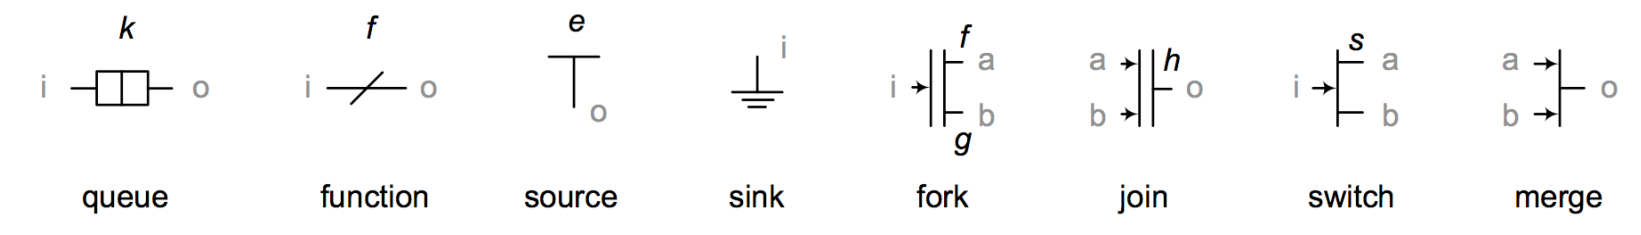
\includegraphics[width=1.0\textwidth]{xmas-language}
\caption{Eight primitives of the xMAS language \cite{6225465}. Italicized letters indicate
parameters. Gray letters indicate ports.}
\label{fig:xmas-language}
\end{figure}

\paragraph{Design and verification tools}

To make use of the xMAS language and verification tools, computer scientists
have developed an application called WickedXMAS \cite{WickedXmas}.
With this application it is possible to draw a model and export it so it can be
verified. The verification tool reads the model and processes one or more
algorithms e.g. to detect network deadlocks or model syntax faults.

Although the WickedXMAS designer tool is still useful and unique in its kind
there are some major shortcomings and had to be redesigned because:
\begin{enumerate}
\item It was written in csharp which makes it only available for researchers
working on a Windows platform.
\item Verification tools are not integrated which
makes it complicated to use.
\item The model must be exported before it can be
used by the verification tools.
\item It is difficult to maintain, verification tools are written in c++ while
designer is written in csharp and xaml
\item The tool aborts in several situations.
\item Lack of composite management.
\item Recursive composite feature not working.
\end{enumerate}

Therefore our team was asked to design and build a new tool. Our goal was to
create a maintainable, platform independent, xMAS modeling tool that integrates
the verification tools.
By integrating formal verification into a new designer-friendly tool, a designer
can easily verify a design.

The project is split into a designer that we call
``xmd'' or xMAS Model Designer and the verification process called ``xmv'' or
xMAS Model Verification. The project is based on Qt's latest technology where we
have written the GUI in QML (JavaScript) and the logic in c++.

Instead of implementing specific verification tools we have put our effort into
implementing a generic plug-in interface. Via this interface, verification tools
can be easily plugged in and controlled. This interface can also send the
verification results to the console.
\begin{wrapfigure}{r}{0.55\textwidth}
  \vspace{-20pt}
  \begin{center}
    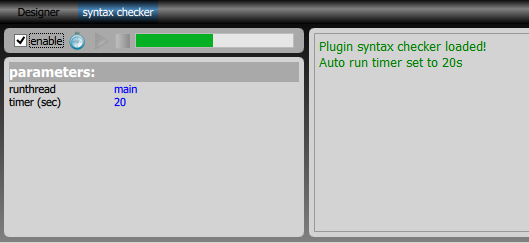
\includegraphics[width=0.50\textwidth]{console}
  \end{center}
  \vspace{-20pt}
  \caption{xmd syntax checker plug-in console}
  \label{fig:console}
  \vspace{-10pt}
\end{wrapfigure}
A scientist can easily implement a new verification algorithm if it has the
plug-in interface. We have provided the syntax checker of such a plug-in interface
that can be used as an example for other verification tools. Each plug-in
automatically gets its own console output and control with setup fields.
Starting a verification process is simply done by clicking the start button, no
conversion or exports are necessary anymore.


In the new designer ``xmd'' all actions on the canvas are now directly reflected
into the model network and can be verified immediately. Another improvement of
the designer is the management of composite components, which are subnetworks
that can be reused and make it possible to quickly build large models in an easy
way.
\begin{wrapfigure}{r}{0.55\textwidth}
  \vspace{-20pt}
  \begin{center}
    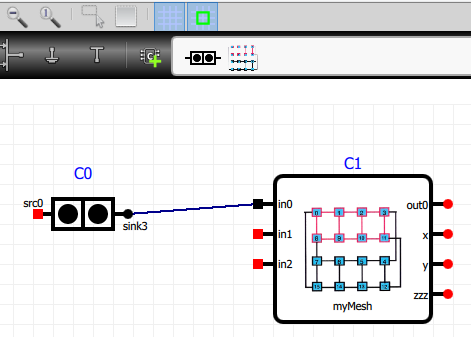
\includegraphics[width=0.50\textwidth]{composite-use}
  \end{center}
  \vspace{-20pt}
  \caption{xmd composite library and canvas use}
\label{fig:composite-use}
  \vspace{-10pt}
\end{wrapfigure}
A model can be setup with composite properties so it can be used just
like a primitive. A designer can do this by adding them to a model its composite
library and drag those into the canvas. The way that xmd implements composites
gives scientists the opportunity to extend these with a parametric expression.
With a parametric expression it is possible to call a composite in a recursive
way and avoid drawing large networks of already valid subnets.

\newpage
\section{State of the art}
ToDo :pick one of; Parametric composites ,  QoS ,liveness verification \cite{6176626} , ...?


\newpage



\bibliography{../05-research-context/rc}

%%\newpage


\chapter{Product manual}

\section{Project setup}
The purpose of this section is to support maintenance of the xmd software.

\begin{itemize}
\item install Qt 5.4.0
\item install Qt Installer Framework 1.5.0
\item install Google test
\item install Git
\item install Latex tool
\item clone xMAS repository
\end{itemize}

Once the project is setup, open $''.../xmas/src/main.pro''$ with Qt Creator.
Set xmdmain as default and build the Qt project.

\section{Installer}
The purpose of this section is to support xmd end users who want to design and verify xMAS models.

Go to the xMAS web page and download the appropriate installer. For example,
choose $''xmd-win-x86-1.0.0.exe''$ for a 32bit MS Windows platform. After
the download was successful, run the installable and follow the procedure.
If the installation is finished, xmd can be started via the desktop icon or the start menu.

\begin{tcolorbox}[colback=white]
\textbf{
At the moment there is only a Windows installer available and can be found in
the ``installers'' map of the xmas repository.
}
\end{tcolorbox}

\section{xMAS model design}
This section starts with explaining the main parts of the user interface.
Followed by an explanation of the settings and finally how to create and save an
xMAS model.

\subsection{Main window}
Figure~\ref{fig:mainwindow} is the main window of the designer application. On
top there is the xMAS toolbar while in the center it has a single page canvas
that can be setup. A tabbed console can be found at the bottom, the first tab
selects the designer console. Every verification tool loaded as plug-in will get a
console with control panel that can be selected via a tab named as the plug-in.

\begin{figure}[here]
\begin{center}	
	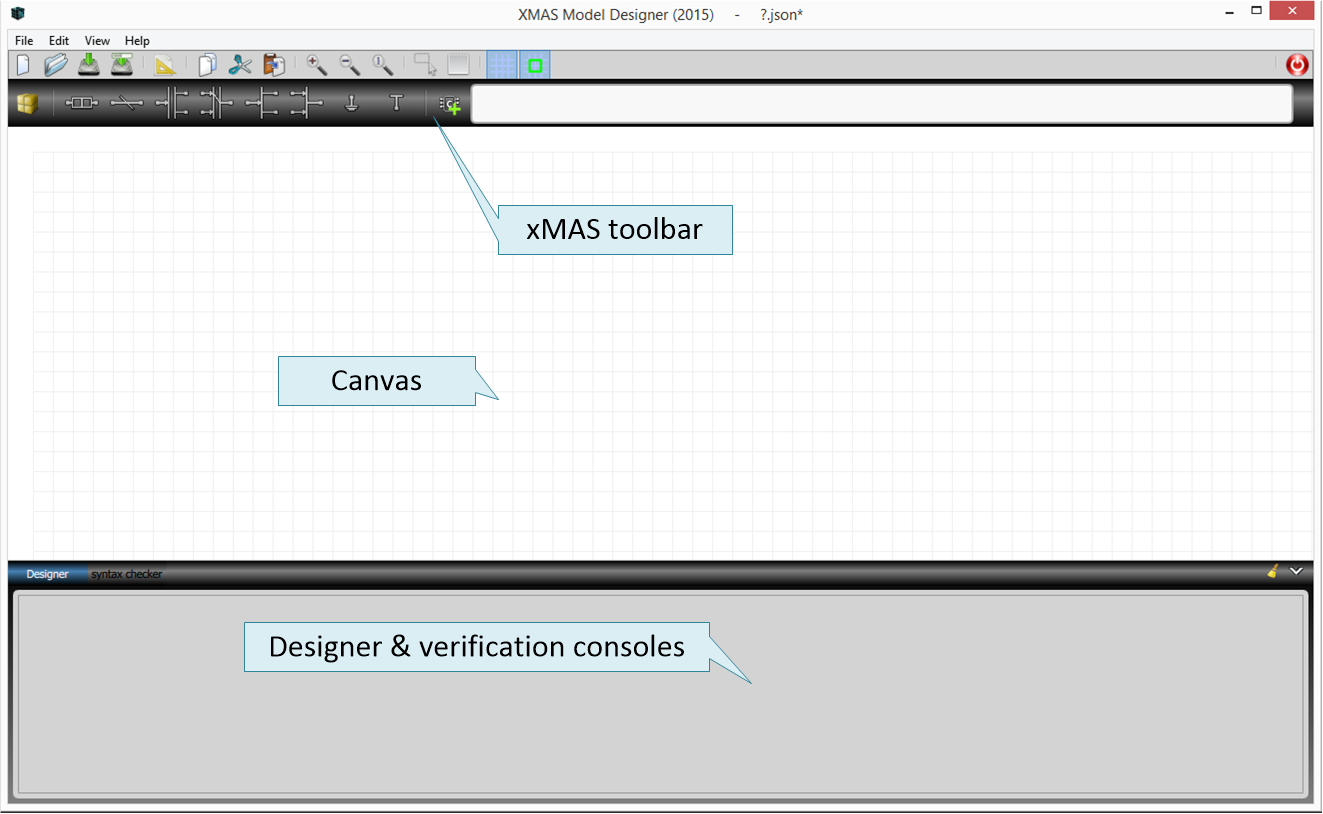
\includegraphics[width=.70\linewidth]{pictures/xmd-empty}
	\caption{Main application window}
	\label{fig:mainwindow}
\end{center}
\end{figure}

\subsection{xMAS tool bar}
The xMAS toolbar (figure~\ref{fig:xmas-toolbar}) holds the items that can be
used to create a model. The packet setup button opens a dialog to set up the
model packet. The xMAS language has only eight primitive components and can be
found next to the packet button. 

\begin{figure}[here]
\begin{center}	
	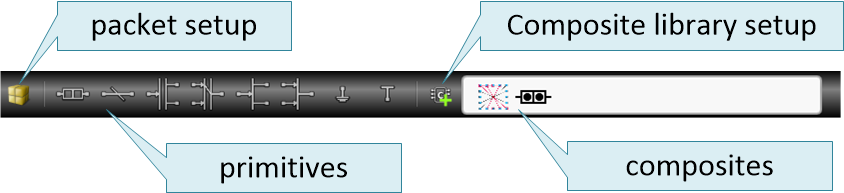
\includegraphics[width=.70\linewidth]{pictures/xmas-toolbar}
	\caption{xMAS toolbar}
	\label{fig:xmas-toolbar}
\end{center}
\end{figure}

Composite components can be found at the right part of this toolbar. Primitive
and composite components can be placed on the canvas by dragging. The area
holding the available composites is called the library which is a horizontal
flickable list. The button at the left side of this list opens a dialog to add a
composite to the library. To remove a composite simply right click the composite
and select remove. Notice that a composite can only be removed if it is not
used.


\subsection{Canvas}
The canvas is a flickable single page, the actual view port can be changed by
drag or swipe it. The size of the canvas page can be changed in the model setup
dialog and is saved with the model. The minimum size is 500 by 500 while the
maximum size is 5000 by 5000. This means that the largest models can directly
hold 500 normal scaled primitive components or 2000 if small scaled.

\paragraph{With grid and snap}canvas items can be easily aligned. The main
toolbar has two toggle buttons, one to show or hide the canvas grid and one to
set the grid snap ``on'' or ``off''. 

\begin{figure}[here]
\begin{center}	
	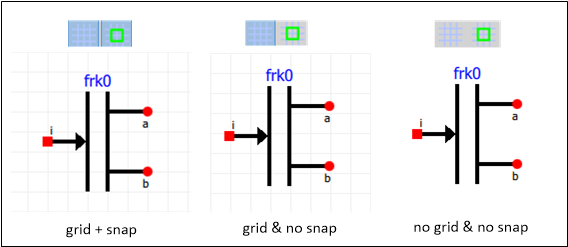
\includegraphics[width=.70\linewidth]{pictures/canvas-grid}
	\caption{canvas grid \& snap options}
	\label{fig:canvas-grid}
\end{center}
\end{figure}

By setting grid snap off a designer can place or move canvas items freely. If
setting this option to ``on'', then at least one component port will snap to the
grid and cannot be placed somewhere in between.

\paragraph{Selecting}canvas items can be done one by one or via a group select.
A selection can be deleted or moved within the canvas its bounds. To select a
group of canvas items you must enable the `group select'' button in the main
toolbar. This because the canvas page its drag-default is used for scrolling.
If group select is enabled then the canvas drag or swipe is disabled.

\begin{figure}[here]
\begin{center}	
	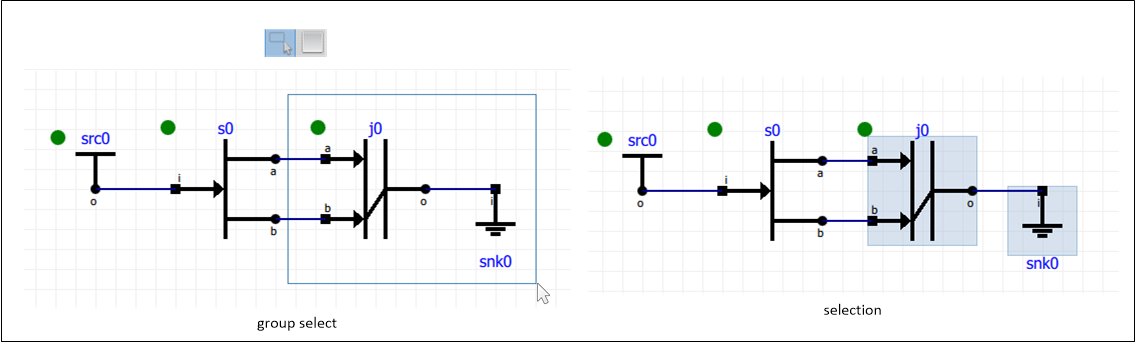
\includegraphics[width=.70\linewidth]{pictures/canvas-selection}
	\caption{canvas group select}
	\label{fig:canvas-selection}
\end{center}
\end{figure}

Next to the ``group select'' button there's a ``select all'' button which selects all
canvas items. Of course all of these actions can be used with standard
shortcuts. Pressing the escape key or click outside the selection will deselect the group.

\paragraph{All components}have common and specific properties. A component
has a name and must be unique. When a component is dragged to the canvas it will
automatically get a unique name. The name can be changed by clicking on it and
press enter when ready. If the name is invalid the change will be ignored. Other
common properties are component size and orientation. Size can be changed in
five steps from 25\% to 400\%. Orientation can be up, down, left and right. Size
and orientation can be set via the context menu or press the left mouse button
and scroll the mouse wheel while hold the ``Ctrl'' or ``Alt'' key. Of course the
touch pad can be used too.

\begin{figure}[here]
\begin{center}	
	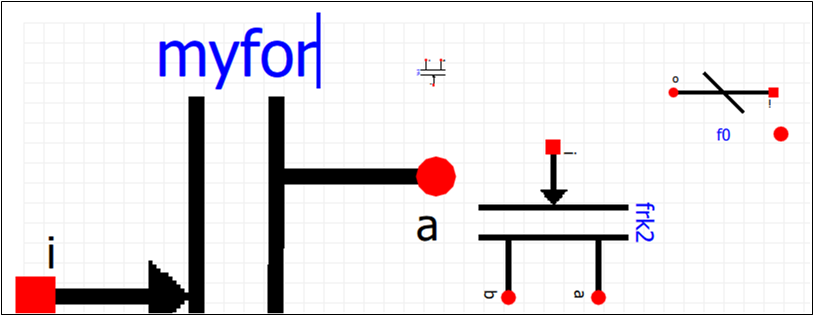
\includegraphics[width=.70\linewidth]{pictures/component-common-properties}
	\caption{canvas common component properties}
	\label{fig:component-common-properties}
\end{center}
\end{figure}

In figure~\ref{fig:component-common-properties}: In-place name editing in
action, small and large size components plus several orientations options are
illustrated. It is also possible to hide or show the component or port names.
These options can be found in the main toolbar or via the canvas context menu.

In figure~\ref{fig:primitives} the graphical representation of the eight
primitive components. Some have a red dot meaning that this component has an
expression to set up. If the expression is valid the dot becomes
green. To open the expression dialog double click on the dot or select it in the
context menu. More information of the expression dialog can be found in the
dialog section~\ref{sec:expression-dialogs}.

\begin{itemize}
\item Queue: In-place size property, a user can only enter digits.
\item Function: Needs a function expression.
\item Fork: No specific properties
\item Join: Need a token expression. Enter 0 or 1 selects the appropriate
input as a restrictive join, otherwise it becomes an unrestrictive join.
\item Switch: Needs a switching expression.
\item Merge: No specific property
\item Sink: Default set as required. A required sink has to be defined later, e.g. outside the composite network.
\item Source: Same as sink but also needs a source expression.
\item Composite: Can be setup with a parametric expression.
\end{itemize}

\begin{figure}[here]
\begin{center}	
	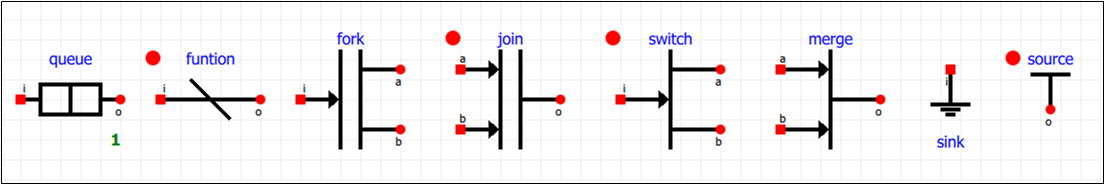
\includegraphics[width=.70\linewidth]{pictures/primitives}
	\caption{list of primitive components}
	\label{fig:primitives}
\end{center}
\end{figure}

\paragraph{A composite} \label{sec:composite} its graphical representation
depends on its model settings, required sinks and sources. If a model is used as
a composite component then all required sinks become outputs and all required
sources become inputs. In other words if a composite network has four required
sinks and three required sources the composite component will have three input
ports at the left and four output ports at the right. In the model setup a user
can also define composite properties. This sets the model its appearance on the
canvas if used as a composite component:
\begin{itemize}
\item The alias is a model nickname and printed in the composite body box.
\item Image is used as a symbol for the composite its body. 
\item If boxed is checked the composite body outline is visible.
Uncheck boxed to let a composite appear as a primitive.
\end{itemize}

\begin{figure}[here]
\begin{center}	
	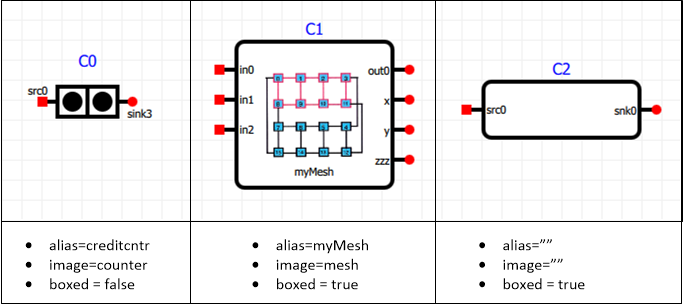
\includegraphics[width=.70\linewidth]{pictures/composites}
	\caption{Composite properties}
	\label{fig:composites}
\end{center}
\end{figure}

The composite at the left in figure~\ref{fig:composites} is un-boxed. For the un-boxed
version the alias will not be printed on the canvas.\\

\begin{tcolorbox}[colback=white]
\textbf{
The symbol for an un-boxed composite must match the default port alignment.
The width is 100 while port spacing is 30.
}
\end{tcolorbox}
\vspace{0.1cm}
The alias is also used as a toolbar tool tip otherwise the filename of the
model-behind is used. A composite that has no symbol gets a default symbol. The
composite at the right in figure~\ref{fig:composites} shows the appearance if no
composite properties were set. A user can always open the composite network and
change its properties. The composite will appear with its new properties in new
and even in existing models.

The port names of a composite are the names of its required sinks and sources.
\begin{tcolorbox}[colback=white]
\textbf{
Try to avoid too long sink and source names so these will fit into the composite its body.
}
\end{tcolorbox}




\subsection{Dialogs}
This subsection gives an overview of all the application specific dialogs. Other
dialogs, e.g. to open or save a model, are native and do not need any further
explanation.
Most dialogs accept with the enter key and cancel with the escape key.

\paragraph{With the application setup dialog} in figure~\ref{fig:app-setup} a
user can change the default model folder. The default model folder is
``xmas-models'' in the users ``home'' directory. A user can select if the
application ask a quit confirm or not. The auto save option will automatically
save the actual modified model every 5 minutes. All these settings are
persistent.\\

\begin{tcolorbox}[colback=white]
\textbf{
It is important to know that models used as composites must be in the same
directory as the main model.
}
\end{tcolorbox}
   
\begin{figure}[t]
\begin{center}	
	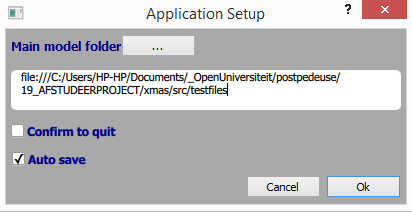
\includegraphics[width=.70\linewidth]{pictures/app-setup}
	\caption{Application setup dialog}
	\label{fig:app-setup}
\end{center}
\end{figure}

\paragraph{The model setup dialog}is used to set the canvas size and the model
filename. Models are saved in json format and therefor the filename must end
with ``.json''. The inputs are checked if valid or not and if not a red border
appears on the entry field. Normally a user does not have to change the folder
because this is set to the application default model folder. But it can become
handy if the user has a sub folder for this modeling project. Composite
properties are optional but useful if this model is meant to be used as a
composite later. Details can be found in the composite paragraph in
section~\ref{sec:composite}. Model size and composite properties are saved in
$''[folder]/[filename]''$. The model setup is shown in
figure~\ref{fig:model-setup}.


\begin{figure}[here]
\begin{center}	
	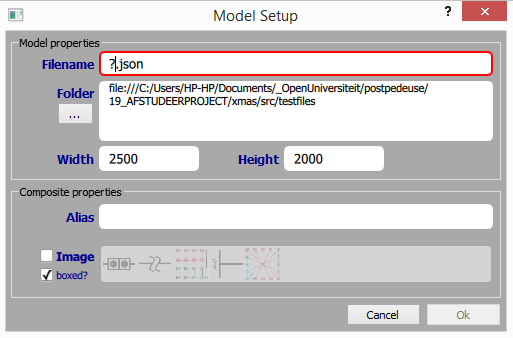
\includegraphics[width=.70\linewidth]{pictures/model-setup}
	\caption{Model setup dialog}
	\label{fig:model-setup}
\end{center}
\end{figure}

\paragraph{The packet setup dialog} is a simple text field entry. It is used to
enter a packet field-range list. The packet is also saved in the model file.
Every field-range entry must start on a new line while field and range are separated with ``\textless ``.
The packet dialog is shown in figure~\ref{fig:packet-setup}.
   
\begin{figure}[here]
\begin{center}	
	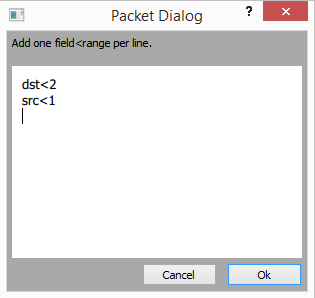
\includegraphics[width=.30\linewidth]{pictures/packet-setup}
	\caption{Packet setup dialog}
	\label{fig:packet-setup}
\end{center}
\end{figure}


\paragraph{Expression dialogs} \label{sec:expression-dialogs}
are used for components that must be set up with
an expression. An expression has a small help on top explaining the syntax and
can differ for each component type. Each time an expression is checked by the
parser and if valid the background becomes green. If the expression is invalid
the background becomes red. The parser will also select the first invalid
character in the expression. A dialog having an invalid expression cannot be
closed with ``ok'' and so not accepted. The expression dialog is shown
in figure~\ref{fig:expression-dialog}.

\begin{figure}[here]
\begin{center}	
	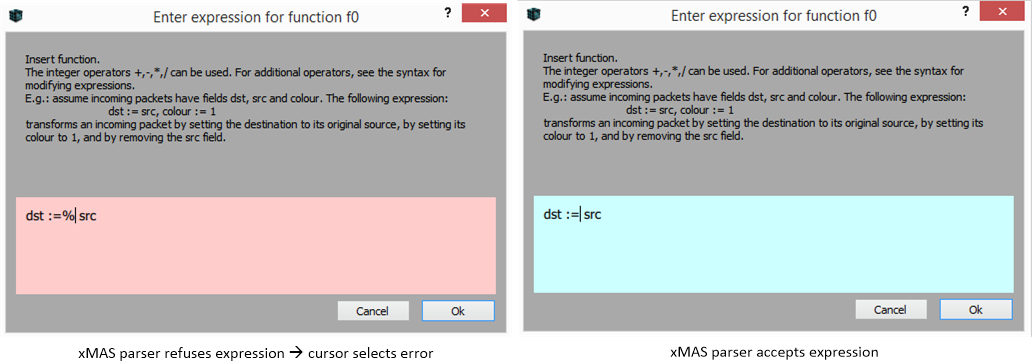
\includegraphics[width=.90\linewidth]{pictures/expression-dialog}
	\caption{Expression dialog}
	\label{fig:expression-dialog}
\end{center}
\end{figure}



\subsection{Designer console}
The designer console is used to print model feedback. The console can be
collapsed, sized or cleared. In figure~\ref{fig:designer-console} you can see an
example of how the expression parser has printed two error messages.

\begin{figure}[here]
\begin{center}	
	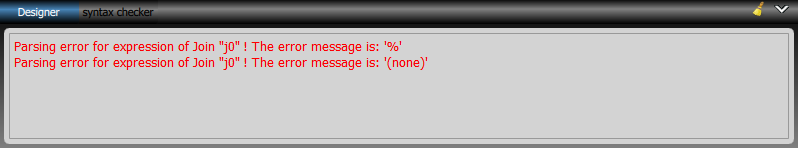
\includegraphics[width=.70\linewidth]{pictures/designer-console}
	\caption{Designer console}
	\label{fig:designer-console}
\end{center}
\end{figure}


\section{xMAS model verification}

The new xMAS designer has a plug-in interface to integrate verification tools.
If a verification tool is build as plug-in then it can be loaded and used from
the xMAS designer. The plug-in interface has a generic structure that can be
implemented into each verification tool. The interface provides:
\begin{itemize}
\item a start signal
\item a stop signal
\item a progress value
\item plug-in specific parameters
\item model reference
\item structured or non-structured text messages
\end{itemize}

Structured messages will not be print on the plug-in console but can be parsed as
in-model-feedback.

To support developers of how to implement the interface into their verification
tools the syntax-checker plug-in can be used as an example. If a verification
tool has the interface, than copy the dll file to the plug-in directory of the
xMAS designer. When the xMAS designer starts it will automatically load all valid
plug-ins from the plug-in directory. Each plug-in will get a console tab.
Figure~\ref{fig:plug-in-console} has one for the syntax checker.

\begin{figure}[here]
\begin{center}	
	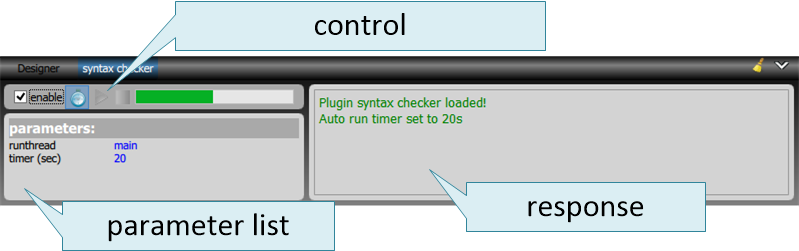
\includegraphics[width=.70\linewidth]{pictures/plug-in-console}
	\caption{Plug-in console}
	\label{fig:plug-in-console}
\end{center}
\end{figure}

\begin{tcolorbox}[colback=white]
\textbf{
In the current project, only the syntax checker has a plug-in interface and can
be used within the designer.
}
\end{tcolorbox}

\paragraph{The plug-in console}has three UI items :
\begin{itemize}
\item The control panel
\item The parameter list
\item The repose list
\end{itemize}

With the control panel a user can send a start or stop to the plug-in. The start
can also triggered by a timer, set by the plug-in interval parameter. For
example in the parameter list of the syntax checker we see that it will run in
the main thread and that it is time triggered every twenty seconds. The control
panel panel also has a progress bar. The parameter list shows all the plug-in
its specific parameters and are read via the interface.

\begin{tcolorbox}[colback=white]
\textbf{
At the moment plug-in parameters cannot be edited via the designer.
}
\end{tcolorbox}


\section{Remarks}
\begin{itemize}
\item The bug list can be found in the appendix or in the Agilefant backlog.
\item The fix list can be found in the appendix or in the Agilefant backlog.
\item Possible features can be found in the appendix or in the Agilefant backlog.
\end{itemize}


\chapter{System Documentation}
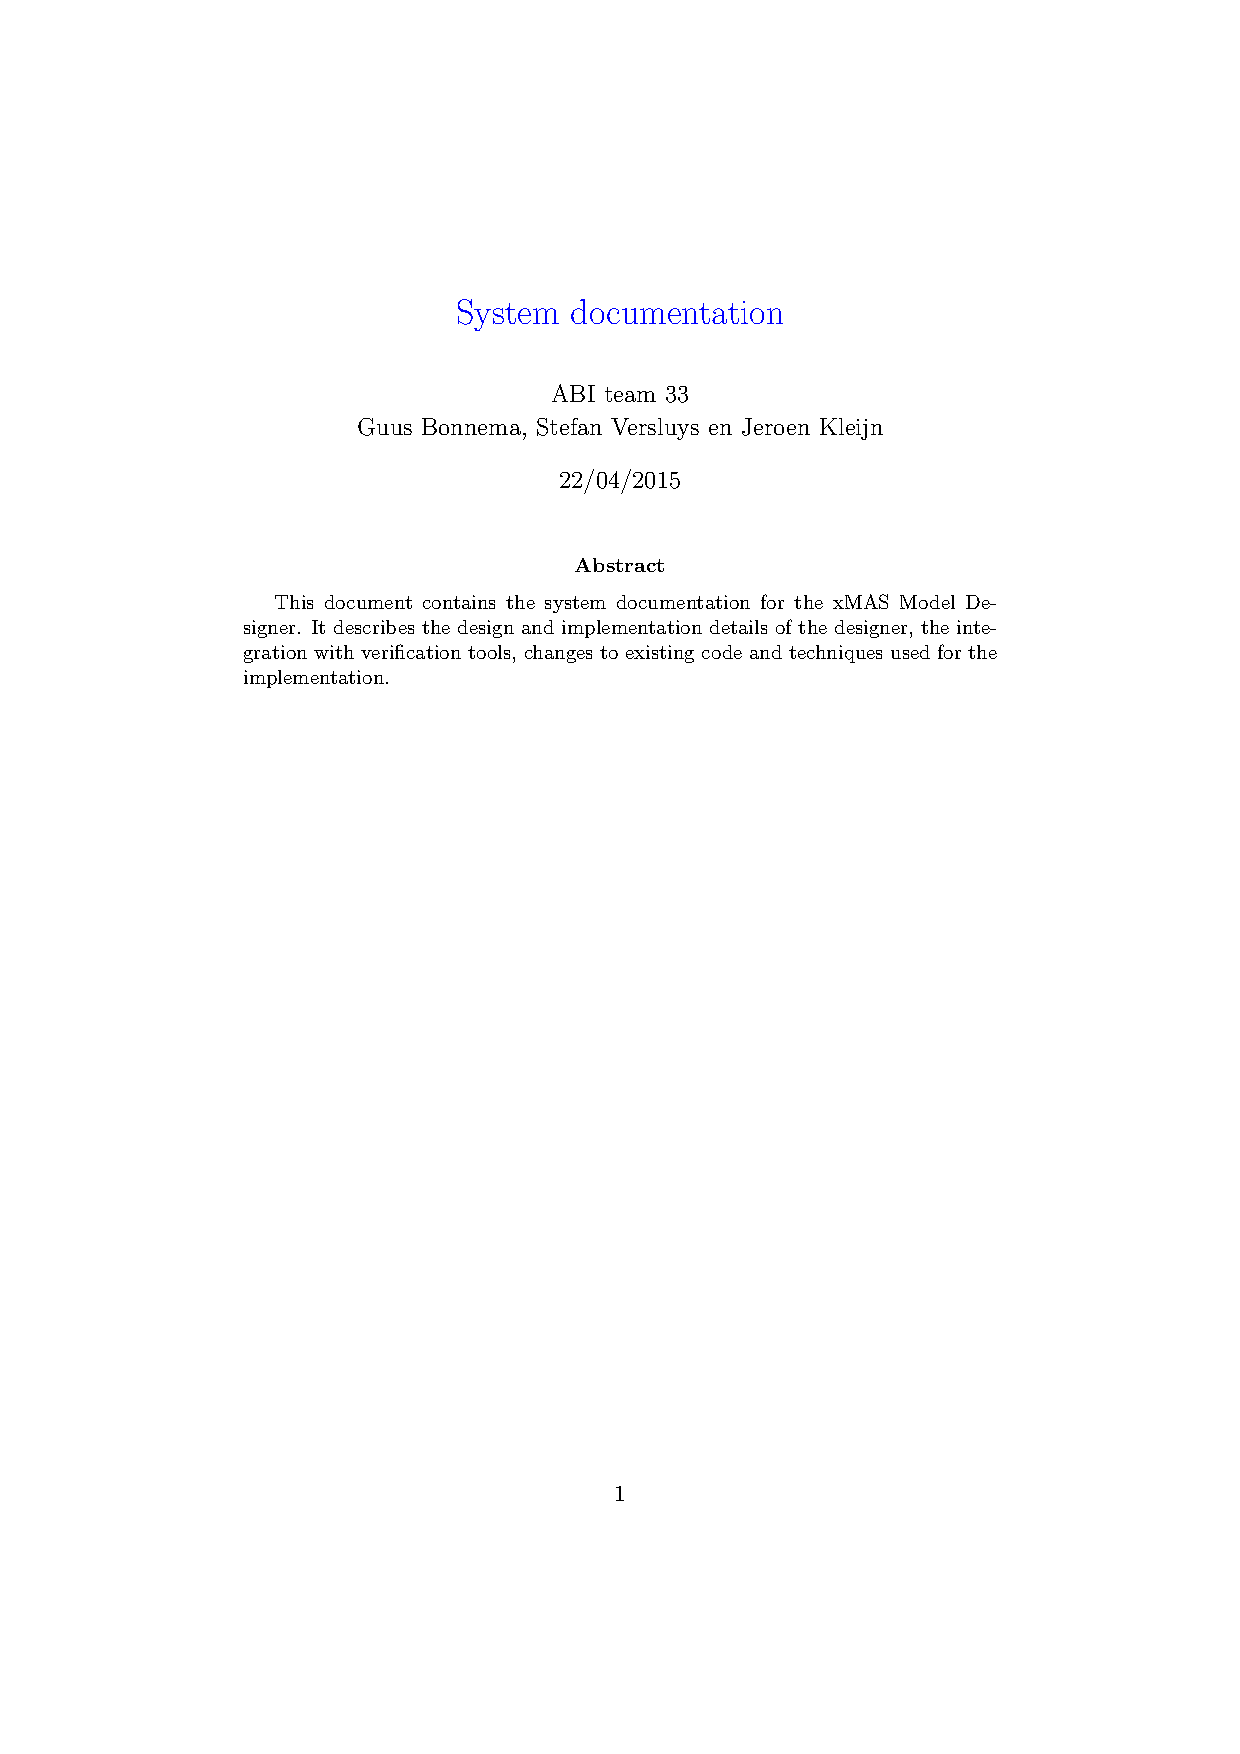
\includepdf[pages=-]{../09-appendix/system-docs.pdf}



\section{section1}
\todo[inline]{
individueel verslag onderzoek deeldomein en bijhorende technieken, plusminus 5 pagina's
}
%%\newpage


\chapter{Reflection}
\paragraph{Project} We started out largely unsure about how to continue. The first few months
planning we structured internal and external communication. Additionally, we decided to 
work in time boxes (iterations) where we successively worked toward a finished project. 
The internal communication was intense (three times a week, sometimes more) where one of our
members routinely worked more hours at the office in order to join our call. The division of work 
was partly pre-agreed upon and partly just happened.

Right after the first iteration we encountered the first problem: our mentor for the project 
and the customer both ceased to respond to our mails. Being December, we figured they were 
on an unscheduled holiday. About a month later (half of January) the customer explained 
what was happening. The mentor was sent off to the U.S. and our customer's workload had been 
increased to a level where he hardly had the chance to join us in a call. This was all due to 
a reorganization within the Open University. The OU was retiring approximately 10 - 30\% of their
personnel\footnote{When we commented on this during the midterm review, the OU people present,
did not feel the students needed to know. Apparently, our team was the only team impacted 
by the change. Still we wonder why such a large reorganization was not communicated broadly, 
even if most of the students should not notice anything, after all: it's a big change.}.
 
We realized we had to change our approach. Although initially we talked about rescheduling,
we decided not to. One of the advantages of agile working is the principle of the time-box. 
The consequent of the decrease of communication with the customer would be a decrease in speed
of deciding. We agreed with the customer to have at minimum one skype session per iteration. 
This we added to our planning. Informally, we could request a quick answer to urgent questions
by email.

In conclusion we finished our product more or less as we planned to. We had initially
hoped to have covered more ground, but in the circumstances we are quite content with what 
we produced. The customer and the mentor expressed contentment as well.

\paragraph{Product} The product turned out more or less as we envisioned at the start. The one
thing we might do differently in hindsight, is to spend a little more attention to the decision
of using a tight integration with the existing xmas programs that were developed before we started.

The issue was whether to use a text interface causing complete segregation of user interface and
xmas programs, or, to use a tight interface to the xmas programs. The customer chose the tight 
interface fearing the consequences of a second parser for maintenance. We chose to integrate
\qml and \cpp which probably cost about 2 iterations (6 weeks) extra in comparison to a text
interface. Although this is partly conjecture, if the team and the customer had known the extent 
of the consequences, we might have chosen differently.

\paragraph{Guus} I felt very happy working this project with a very intense communication pattern,
a positively constructive team and supportive and helpful mentor and customer. I started out 
unfamiliar with the agile way of working and ended up liking the way it works. 
Especially the time box turned out very useful when events 
turned against us. In a planned environment, where functionality is fixed and time variable, I 
am convinced we would have had to reschedule our project. I am very glad we chose to go agile.

Learning \cpp was a real pleasure, although my work managing stuff took a large part of my time,
especially during planning and preparing for our meetings. Additionally, once we started programming,
all time I wanted to spend on learning \cpp evaporated. My connotation of \cpp has significantly improved
due to the working with live \cpp programs.

I also learned the impact of strictness in an agile project. Too much strictness stiffles initiative 
and creativity. However, some strictness is necessary to constantly know where we are and what we 
still need cover in order to succeed.

Agile and strictness is a troubled marriage at best. I am very glad to have learned this valuable lesson and
I am grateful to my team mates who endured my overload of control and finally corrected me when I was 
enforcing too much.

\paragraph{Jeroen}
todo \\ 
\todo[inline]{reflection jeroen}

\paragraph{Stefan: }
From time to time I thought that it would be difficult to reach our targets so
we could meet the customer requirements. After all we had to start from scratch
and with a limited amount of time. It took some time to find the right platform
independent tools plus we had to understand the complex context and think about
solutions for new features. So we had to do a lot of research before we could
start writing a single line of code. Even though we weren't familiar with some
technologies we always tried to pick the best options instead of picking quick
\& cheap.

Meeting our goals and learning new technologies was one thing but I also wanted
to try out an agile approach. I can't say if DAD was the right choice or not,
but I would recommend DAD to anyone who want to start practicing agile methods.
This because DAD can be tailored by the needs and it does not prescribe strict
rules but is rather people and learning oriented.

One of the suggested DAD practices that was important for our distributed team
was how to ``visualize work''. For that purpose we chose Agilefant which is an
open source web based agile management tool. I'm very satisfied about this kind
of tools, it has a little bit of learning curve but you get quickly much in
return. A tool like Agilefant reduces the disadvantage of a distributed team
compared to a co-located teams. Many times we've used it to lead our on-line
meetings so we could align our thoughts. Together with on-line communication
tools I think this is a must have for distributed agile teams.

As for anyone else we also had to deal with ups and downs, technically and
personally. The most important thing is that we all were there to help or
listening whenever it was necessary. We communicated a lot and it was rarely
that someone was not available and in my opinion this was also our strength that
we managed to quickly find a solution and kept motivation.

After nine months of hard working, I can say that I'm very happy about the
result and the experience. I could increase my skills in new technologies more
as expected. I could also practice agile methods and learn how these contribute
in reaching goals. Finally and last but not least, all of this wouldn't be possible
without the support and effort of Guus and Jeroen.

\chapter*{Conclusion}
\todo[inline]{conclusion  --> in progress, text wil be based on our feature list in the appendix}

\begin{tcolorbox}[colback=yellow!30]
Freek $\rightarrow$ \\
 Conclusie: Hier kun je onder andere wat "future work" kwijt. Hoe zouden jullie jullie tool verder ontwikkelen. Stel we hebben een nieuw ABI groepje, wat zou deze kunnen doen en wat raden jullie hun aan? Staar je niet blind op pagina nummers, 1 pagina is ook goed.
\end{tcolorbox}

%%\newpage



\appendix
\chapter{Appendix}
\section{Bug list}
\begin{enumerate} \label{sec:bug-list}
\item	Invalid maximized main window restore from setup (Qt Bug)
\item	Group select has not always key focus (e.g. pressing delete has no effect)
\item	Several memory leaks
\item Error when building release version
\item Windows warning : Some dialogs do not get destroyed before quit (see Agilefant details)
\item	\st{No model modified flag when packet changed}
\item	\st{Packet dialog not cleared on new/open network}
\item \st{Not able to enter an empty packet}
\item	\st{Model modified flag set after new when canvas was not clear}
\item	\st{Clicking new if canvas is not clear aborts application under Linux.}
\item	\st{Model setup not restored on model open.}
\item \st{With composite on canvas and click new then dialog save first $+$ no does not
work}
\item \st{Sometimes a composite its mouse area becomes inactive. (start with a clean
canvas , add a composite in the library and drag one on the canvas. Save new
model and click new or open). This only occurs with new (nameless) networks,
adding a composite is probably not handled well in the xMAS networks list and
therefore do only exists on the canvas.}
\item \st{Qt warning ``QObject::connect: signal not found in Logger'' (windows)}
\end{enumerate}


\section{Fix list}
\begin{enumerate}\label{sec:fix-list}
\item	Grid snap on port center instead of component body left top
\item	Grid snap when drag a group of items
\item	Qt save as dialog not available in version 5.4.0
\item QML uses non blocking calls, cannot use yes/no dialogs feedback in a
proper way.
\item Use of destroy dialog to quit application from QML dialog to prevent
Windows warning (Qt bug).
\item Allow entering source expression when not connected (xmas parser)
\item New page is now done by select all and delete, instead destroy page and
create new page.
\item Remove qml convert logic in network.cpp, instead send a add component
request to the canvas by its name and type. Signal the update to component.cpp
which already does the request to xMAS for the other properties like x,y,… This
to avoid duplicate conversion and checks.
\item	\st{Tooltip for composites in library to show alias or filename}
\item	\st{Tooltip for primitives in toolbar}
\end{enumerate}


\section{Feature list}

\paragraph{features}
\begin{enumerate}
\item	(x,y) anchor list to draw a channel via these points
\item	Pathfinder algorithm for channels (e.g. A*)
\item	Canvas scroll while drag items
\item	Canvas copy-cut-paste
\item	Canvas undo-redo
\item	Canvas rotate group selection
\item	Redirect standard output to the plug-in consoles
\item	Plug-in parameters change read-only to editable list
\item	Replace auto plug-in load from fixed folder to add/remove
\item	Model export
\item	Parametric composite
\item	Packet editor as editable key/value list
\item	Plug-in tools add progress value.
\item	Plug-in tools add stop process. 
\item	Deadlock checker with plug-in interface
\item	Plug-in structured text for “in model” feedback
\item Channel rewire via clicking a connected port. (no you need to delete and
create new channel)
\item	Multi page model editor
\item	Open composite sub network in main model (e.g. on a new page)
\item	Application help
\item A platform dependent binaries package of the Qt project so that user can
install the application without having Qt or other tools installed.
\end{enumerate}


% Bibliography ---> need to include
\bibliography{tr}

\end{document} ;########################### end document ##################################;
